\documentclass[11pt, a4paper]{article}

% Mandatory Packages
\usepackage{amsmath}
\usepackage{amssymb}
\usepackage{amsthm}
\usepackage{geometry}
\usepackage{tikz}
\usetikzlibrary{arrows.meta, positioning, shapes, patterns}
\usepackage{mathrsfs}
\usepackage{mathtools}
\usepackage{hyperref}

% Page Geometry
\geometry{top=1in, bottom=1in, left=1in, right=1in}

% Theorem Environments
\newtheorem{theorem}{Theorem}[section]
\newtheorem{lemma}[theorem]{Lemma}
\newtheorem{proposition}[theorem]{Proposition}
\newtheorem{corollary}[theorem]{Corollary}
\theoremstyle{definition}
\newtheorem{definition}{Definition}[section]
\newtheorem{axiom}{Axiom}[section]
\newtheorem{example}{Example}[section]
\theoremstyle{remark}
\newtheorem{remark}{Remark}[section]

% Title Information
\title{Homework 4.5: Fundamental Properties of Set Operations}
\author{Tashfeen Omran}
\date{September 2026}

\begin{document}

\maketitle
\tableofcontents
\newpage

% ==========================================
% PART 1: Comprehensive Introduction
% ==========================================
\section{Part 1: Comprehensive Introduction, Context, and Prerequisites}

\subsection{Core Concepts \& Axioms}
The mathematical universe is fundamentally constructed from \textit{sets}---collections of distinct objects considered as an object in their own right. Section 4.5 focuses on the algebraic structure of these sets, specifically how they interact through fundamental operations. 

Let $U$ be a universal set, and let $A, B, C \subseteq U$. We define the core operations as follows:
\begin{itemize}
    \item \textbf{Union ($A \cup B$):} The set of all elements in $A$, in $B$, or in both. Formally, $A \cup B = \{x \in U : x \in A \lor x \in B\}$.
    \item \textbf{Intersection ($A \cap B$):} The set of all elements in both $A$ and $B$. Formally, $A \cap B = \{x \in U : x \in A \land x \in B\}$.
    \item \textbf{Complement ($\overline{A}$ or $A^c$):} The set of all elements in $U$ that are not in $A$. Formally, $\overline{A} = \{x \in U : x \notin A\}$.
    \item \textbf{Set Difference ($A - B$ or $A \setminus B$):} The set of elements in $A$ that are not in $B$. Formally, $A - B = \{x \in U : x \in A \land x \notin B\} = A \cap \overline{B}$.
\end{itemize}

The foundational axiom governing these proofs is the \textbf{Axiom of Extensionality}, which states that two sets are equal if and only if they contain exactly the same elements. Therefore, to prove $X = Y$, we must prove $X \subseteq Y$ (if $x \in X$, then $x \in Y$) and $Y \subseteq X$ (if $x \in Y$, then $x \in X$).

\subsection{Intuition and Set-Theoretic/Logical Foundations}
Set operations are perfectly isomorphic to propositional logic. The union ($\cup$) corresponds to the logical OR ($\lor$), intersection ($\cap$) to AND ($\land$), and complement ($\overline{A}$) to NOT ($\neg$). When we prove set identities, we are essentially "chasing elements" by translating a set statement into a logical statement, applying the rules of Boolean logic, and translating back into set notation. 

\subsection{Historical Context and Motivation}
In the late 19th century, Georg Cantor developed naive set theory, which revolutionized mathematics by providing a common language for all mathematical objects. However, paradoxes (like Russell's Paradox) revealed that defining sets purely by arbitrary properties was logically inconsistent. This crisis led to the rigorous axiomatization of set theory (Zermelo-Fraenkel with Choice, or ZFC). The algebraic properties of sets we study here were heavily formalized by George Boole, whose "Boolean Algebra" showed that logic and set theory obey strict algebraic laws, much like the arithmetic of real numbers.

\subsection{Key Theorems, Lemmas, and Formulas}
\begin{theorem}[Theorem 4.22: Fundamental Properties of Set Operations]
For any sets $A, B$, and $C$ within a universal set $U$:
\begin{enumerate}
    \item \textbf{Commutative Laws:} $A \cup B = B \cup A$ and $A \cap B = B \cap A$.
    \item \textbf{Associative Laws:} $A \cup (B \cup C) = (A \cup B) \cup C$ and $A \cap (B \cap C) = (A \cap B) \cap C$.
    \item \textbf{Distributive Laws:} $A \cup (B \cap C) = (A \cup B) \cap (A \cup C)$ and $A \cap (B \cup C) = (A \cap B) \cup (A \cap C)$.
    \item \textbf{De Morgan's Laws:} $\overline{A \cup B} = \overline{A} \cap \overline{B}$ and $\overline{A \cap B} = \overline{A} \cup \overline{B}$.
\end{enumerate}
\end{theorem}

\subsection{Prerequisites}
To master this section, one must be proficient in:
\begin{itemize}
    \item \textbf{Propositional Logic:} De Morgan's laws for logic ($\neg(P \land Q) \iff \neg P \lor \neg Q$), distributive laws of logic.
    \item \textbf{Direct Proof Techniques:} Specifically, the method of "element-chasing" to prove mutual subset inclusion ($X \subseteq Y$ and $Y \subseteq X$).
    \item \textbf{Set-Builder Notation:} Translating between $x \in A \cap B$ and $x \in A \land x \in B$.
\end{itemize}

% ==========================================
% PART 2: Detailed Homework Solutions
% ==========================================
\section{Part 2: Detailed Homework Solutions (Rigorous Proofs)}

\textit{Note: In accordance with strategic problem selection, we have chosen a representative sample from Section 4.5 (Exercises 4.54, 4.55, 4.57, and 4.59) to cover all distinct problem archetypes: basic identities, set differences, algebraic proofs, and complex nested operations.}

\subsection{Exercise 4.54}
\textbf{Problem:} Prove that $\overline{A \cap B} = \overline{A} \cup \overline{B}$ for every two sets $A$ and $B$ (Theorem 4.22(4b)).

\begin{proof}
\textit{Proof Technique: Direct Proof via Element-Chasing (Mutual Inclusion).}

\textbf{Part 1: Show $\overline{A \cap B} \subseteq \overline{A} \cup \overline{B}$.}
Let $x$ be an arbitrary element such that $x \in \overline{A \cap B}$. 
By the definition of the complement, this means $x \notin (A \cap B)$.
By the definition of intersection, it is not the case that $x$ is in both $A$ and $B$. Logically, $\neg(x \in A \land x \in B)$.
By De Morgan's Law for propositional logic, this is equivalent to $(x \notin A) \lor (x \notin B)$.
By the definition of the complement, this means $x \in \overline{A} \lor x \in \overline{B}$.
By the definition of union, $x \in \overline{A} \cup \overline{B}$.
Since $x$ was arbitrary, we conclude that $\overline{A \cap B} \subseteq \overline{A} \cup \overline{B}$.

\textbf{Part 2: Show $\overline{A} \cup \overline{B} \subseteq \overline{A \cap B}$.}
Let $y$ be an arbitrary element such that $y \in \overline{A} \cup \overline{B}$.
By the definition of union, $y \in \overline{A} \lor y \in \overline{B}$.
By the definition of complement, $y \notin A \lor y \notin B$.
By De Morgan's Law for propositional logic, this is equivalent to $\neg(y \in A \land y \in B)$.
By the definition of intersection, $y \notin (A \cap B)$.
By the definition of complement, $y \in \overline{A \cap B}$.
Since $y$ was arbitrary, we conclude that $\overline{A} \cup \overline{B} \subseteq \overline{A \cap B}$.

Since both subset inclusions hold, $\overline{A \cap B} = \overline{A} \cup \overline{B}$.
\end{proof}

\subsection{Exercise 4.55}
\textbf{Problem:} Let $A, B$, and $C$ be sets. Prove that $(A - B) \cap (A - C) = A - (B \cup C)$.

\begin{proof}
\textit{Proof Technique: Direct Proof via Biconditional Logical Equivalences.}
Instead of splitting into two subset proofs, we can use a chain of logical equivalences ($\iff$), as every step is reversible.

Let $x$ be an arbitrary element in the universal set $U$.
\begin{align*}
    x \in (A - B) \cap (A - C) &\iff x \in (A - B) \land x \in (A - C) \quad &&\text{(Definition of Intersection)} \\
    &\iff (x \in A \land x \notin B) \land (x \in A \land x \notin C) \quad &&\text{(Definition of Set Difference)} \\
    &\iff (x \in A \land x \in A) \land (x \notin B \land x \notin C) \quad &&\text{(Commutativity/Associativity of $\land$)} \\
    &\iff x \in A \land (x \notin B \land x \notin C) \quad &&\text{(Idempotent Law of Logic)} \\
    &\iff x \in A \land \neg(x \in B \lor x \in C) \quad &&\text{(De Morgan's Law of Logic)} \\
    &\iff x \in A \land x \notin (B \cup C) \quad &&\text{(Definition of Union)} \\
    &\iff x \in A - (B \cup C) \quad &&\text{(Definition of Set Difference)}
\end{align*}
Because the logical statements are equivalent at every step, the sets contain exactly the same elements. Thus, $(A - B) \cap (A - C) = A - (B \cup C)$.
\end{proof}

\subsection{Exercise 4.57}
\textbf{Problem:} Let $A, B$, and $C$ be sets. Use Theorem 4.22 to prove that $\overline{A \cup (B \cap C)} = (\overline{A} \cap \overline{B}) \cup (\overline{A} - C)$.

\begin{proof}
\textit{Proof Technique: Algebraic Set Manipulation.}
Here, we do not chase elements. We apply the established axioms from Theorem 4.22 directly to the sets.

\begin{align*}
    \overline{A \cup (B \cap C)} &= \overline{A} \cap \overline{(B \cap C)} \quad &&\text{(De Morgan's Law for Union)} \\
    &= \overline{A} \cap (\overline{B} \cup \overline{C}) \quad &&\text{(De Morgan's Law for Intersection)} \\
    &= (\overline{A} \cap \overline{B}) \cup (\overline{A} \cap \overline{C}) \quad &&\text{(Distributive Law of $\cap$ over $\cup$)}
\end{align*}
Recall the definition of set difference: for any sets $X$ and $Y$, $X - Y = X \cap \overline{Y}$. 
Applying this to the second term, we have $\overline{A} \cap \overline{C} = \overline{A} - C$.
Substituting this back into our equation yields:
\[
    \overline{A \cup (B \cap C)} = (\overline{A} \cap \overline{B}) \cup (\overline{A} - C)
\]
This completes the proof.
\end{proof}

\subsection{Exercise 4.59}
\textbf{Problem:} Show for every three sets $A, B$, and $C$ that $A - (B - C) = (A \cap C) \cup (A - B)$.

\begin{proof}
\textit{Proof Technique: Algebraic Set Manipulation.}

We begin with the left-hand side and apply the definition of set difference, $X - Y = X \cap \overline{Y}$.
\begin{align*}
    A - (B - C) &= A \cap \overline{(B - C)} \quad &&\text{(Definition of Set Difference)} \\
    &= A \cap \overline{(B \cap \overline{C})} \quad &&\text{(Definition of Set Difference)} \\
    &= A \cap (\overline{B} \cup \overline{\overline{C}}) \quad &&\text{(De Morgan's Law)} \\
    &= A \cap (\overline{B} \cup C) \quad &&\text{(Double Complement Law)} \\
    &= (A \cap \overline{B}) \cup (A \cap C) \quad &&\text{(Distributive Law)} \\
    &= (A - B) \cup (A \cap C) \quad &&\text{(Definition of Set Difference)} \\
    &= (A \cap C) \cup (A - B) \quad &&\text{(Commutative Law of Union)}
\end{align*}
Thus, $A - (B - C) = (A \cap C) \cup (A - B)$.
\end{proof}

% ==========================================
% PART 3: In-Depth Analysis
% ==========================================
\section{Part 3: In-Depth Analysis of Problems and Techniques}

\subsection{A) Problem Types and Logical Strategies}
The problems in this section fall into two distinct archetypes:
\begin{enumerate}
    \item \textbf{Element-Chasing Proofs (Exercises 4.54, 4.55):} The strategy is to take an arbitrary element $x$ from the left-hand set and logically deduce that it must belong to the right-hand set, and vice versa. This is the most fundamental, rigorous way to prove set equality from the ground up.
    \item \textbf{Algebraic Set Proofs (Exercises 4.57, 4.59):} Once fundamental theorems (like De Morgan's and Distributive laws) are established via element-chasing, we can treat sets like algebraic variables. The strategy here is to substitute definitions (especially $A - B = A \cap \overline{B}$) and factor/expand expressions just as one would in polynomial algebra.
\end{enumerate}

\subsection{B) Key Analytical and Logical Manipulations}
\begin{itemize}
    \item \textbf{The Set Difference Translation:} The most critical trick in Exercises 4.57 and 4.59 is converting $X - Y$ into $X \cap \overline{Y}$. Set difference does not distribute nicely, but intersection does. By converting to intersections and complements, we unlock the ability to use De Morgan's and Distributive laws.
    \item \textbf{Logical De Morgan's vs. Set De Morgan's:} In Exercise 4.54, we explicitly bridged the gap between logic and sets. We used the logical equivalence $\neg(P \land Q) \iff \neg P \lor \neg Q$ to prove the set equivalence $\overline{A \cap B} = \overline{A} \cup \overline{B}$. 
    \item \textbf{Idempotent Law of Logic:} In Exercise 4.55, we encountered $(x \in A) \land (x \in A)$. Recognizing that $P \land P \iff P$ allowed us to simplify the expression and factor out the $A$.
\end{itemize}

% ==========================================
% PART 4: Cheatsheet, Visuals, and Tips
% ==========================================
\section{Part 4: "Cheatsheet", Visuals, and Tips for Success}

\subsection{Theorems \& Equivalences Summary}
\begin{itemize}
    \item \textbf{Set Difference:} $A - B = A \cap \overline{B}$
    \item \textbf{De Morgan's:} $\overline{A \cup B} = \overline{A} \cap \overline{B}$ \quad and \quad $\overline{A \cap B} = \overline{A} \cup \overline{B}$
    \item \textbf{Distributive:} $A \cap (B \cup C) = (A \cap B) \cup (A \cap C)$
    \item \textbf{Absorption:} $A \cup (A \cap B) = A$ \quad and \quad $A \cap (A \cup B) = A$
\end{itemize}

\subsection{Set \& Logic Illustrations}
Below is a Venn diagram illustrating the set $A - (B \cup C)$ from Exercise 4.55. Notice how the shaded region represents elements strictly in $A$, excluding anything that touches $B$ or $C$.

\begin{center}
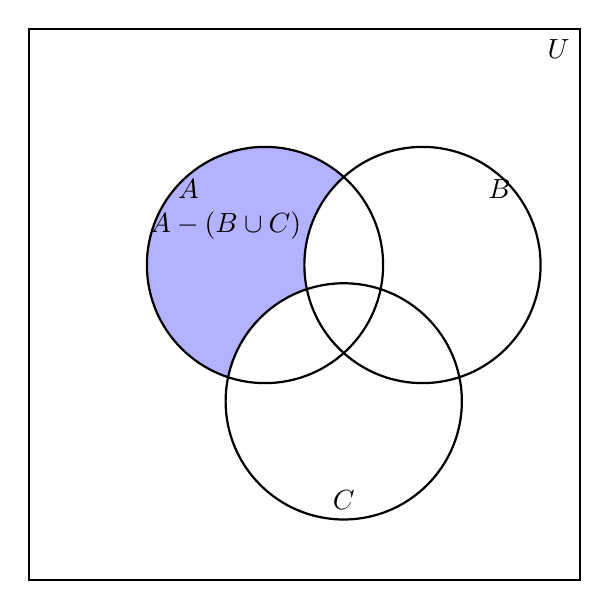
\begin{tikzpicture}[thick]
    % Define the universal set bounding box
    \draw (-3,-4) rectangle (4,3) node[below left] {$U$};
    
    % Shade the region A - (B U C)
    \begin{scope}
        \clip (0,0) circle (1.5cm); % Restrict to A
        \fill[blue!30] (0,0) circle (1.5cm); % Fill A
        \fill[white] (2,0) circle (1.5cm); % Remove B
        \fill[white] (1,-1.732) circle (1.5cm); % Remove C
    \end{scope}
    
    % Draw the outlines of the sets
    \draw (0,0) circle (1.5cm) node[above left=1cm] {$A$};
    \draw (2,0) circle (1.5cm) node[above right=1cm] {$B$};
    \draw (1,-1.732) circle (1.5cm) node[below=1cm] {$C$};
    
    % Label the shaded region
    \node at (-0.5, 0.5) {$A - (B \cup C)$};
\end{tikzpicture}
\end{center}

\subsection{Heuristics \& "Cheats"}
\begin{itemize}
    \item \textbf{When to use which proof?} If a problem contains many set differences ($-$), immediately convert them to intersections with complements ($\cap \overline{B}$) and use algebraic manipulation. If the problem asks to prove a foundational axiom, use element-chasing.
    \item \textbf{The "Distributive" Check:} Just like $2 \times (3 + 4) = (2 \times 3) + (2 \times 4)$, remember that $\cap$ distributes over $\cup$, and $\cup$ distributes over $\cap$. 
\end{itemize}

\subsection{Pitfalls \& Fallacies}
\begin{itemize}
    \item \textbf{Non-Associativity of Set Difference:} A common fatal error is assuming $A - (B - C) = (A - B) - C$. Exercise 4.59 proves this is false. Set difference is \textit{not} associative.
    \item \textbf{Improper Negation:} When element-chasing, writing $x \notin (A \cup B) \implies x \notin A \lor x \notin B$ is a logical fallacy. The correct negation of an OR statement is an AND statement: $x \notin A \land x \notin B$.
\end{itemize}

% ==========================================
% PART 5: Conceptual Synthesis
% ==========================================
\section{Part 5: Conceptual Synthesis and The "Big Picture"}

\subsection{A) Thematic Connections}
The core theme of this chapter is \textbf{Isomorphism}. We are establishing a structural equivalence between Propositional Logic (statements, $\land, \lor, \neg$) and Set Theory (sets, $\cap, \cup, \overline{\phantom{A}}$). Both of these systems are models of a \textit{Boolean Algebra}. By proving these fundamental properties, we show that the rules governing human deduction (logic) are mathematically identical to the rules governing collections of objects (sets).

\subsection{B) Forward and Backward Links}
\begin{itemize}
    \item \textbf{Backward Link:} This topic directly extends Chapter 2 (Logic). We are simply applying truth tables and logical equivalences to a new mathematical object (the set).
    \item \textbf{Forward Link:} This is the absolute bedrock for \textbf{Measure Theory} and \textbf{Probability Spaces}. In advanced probability (Kolmogorov's Axioms), an "event" is a set. The probability of an event, $\mathbb{P}(A)$, requires the space of all events to be closed under countable unions and complements (a $\sigma$-algebra). Without the set-theoretic laws proven here, we could not rigorously define mutually exclusive events or calculate $\mathbb{P}(A \cup B)$.
\end{itemize}

% ==========================================
% PART 6: Abstract Real-World Modeling
% ==========================================
\section{Part 6: Abstract Real-World Modeling (AI, ML, \& Quant Finance)}

\subsection{A) Concrete Scenarios}
\begin{enumerate}
    \item \textbf{Quantitative Finance (Filtrations in Stochastic Calculus):} In pricing derivatives using the Black-Scholes model, we model the stock price as a stochastic process. The information available to a trader at time $t$ is modeled as a $\sigma$-algebra, $\mathcal{F}_t$. As time moves forward, information grows, meaning $\mathcal{F}_s \subseteq \mathcal{F}_t$ for $s < t$. The intersection and union of these sets of events dictate what is mathematically "knowable" at any given time.
    \item \textbf{Machine Learning (Decision Trees and Feature Space Partitioning):} A decision tree classifies data by partitioning the feature space $\mathbb{R}^n$ into disjoint sets. Each split creates a set $A$ and its complement $\overline{A}$. The final leaf node is an intersection of multiple sets (e.g., $A \cap B \cap \overline{C}$). De Morgan's laws are used to optimize and prune these logical rules in algorithms like XGBoost.
\end{enumerate}

\subsection{B) Model Problem Setup: Probability Spaces in Quant Finance}
Let us build a rigorous mathematical model for a one-period binomial options pricing model using set theory.

\textbf{State Space:} Let the sample space of the market be $\Omega = \{\omega_1, \omega_2, \omega_3, \omega_4\}$, representing four possible states of the economy tomorrow.
\textbf{Events ($\sigma$-algebra):} Let $\mathcal{F}$ be the power set of $\Omega$. An event $A \in \mathcal{F}$ is a subset of $\Omega$.
Let $A = \{\omega_1, \omega_2\}$ be the event that Tech stocks go up.
Let $B = \{\omega_2, \omega_3\}$ be the event that Interest Rates go up.

A quantitative analyst wants to price a derivative that pays off only if Tech stocks go down OR Interest rates go down. 
The payoff event is $\overline{A} \cup \overline{B}$.
By De Morgan's Law (Theorem 4.22), we know $\overline{A} \cup \overline{B} = \overline{A \cap B}$.
$A \cap B = \{\omega_2\}$. Thus, the derivative pays off in the event $\overline{\{\omega_2\}} = \{\omega_1, \omega_3, \omega_4\}$.

\textbf{Probability Measure:} We define a risk-neutral probability measure $\mathbb{Q}: \mathcal{F} \to [0,1]$. 
To find the price of the derivative $V_0$, we calculate the expected discounted payoff. If the payoff is $\$1$, then:
\[
    V_0 = e^{-rT} \mathbb{Q}(\overline{A \cap B}) = e^{-rT} \left( 1 - \mathbb{Q}(A \cap B) \right)
\]
This demonstrates how fundamental set operations directly simplify the calculation of derivative pricing in stochastic models.

% ==========================================
% PART 7: Common Variations and Untested Concepts
% ==========================================
\section{Part 7: Common Variations and Untested Concepts}

\subsection{Infinite Families of Sets}
The homework only covers finite operations (unions and intersections of 2 or 3 sets). In advanced mathematics (Topology, Measure Theory), we must deal with \textit{arbitrary} (potentially uncountably infinite) families of sets.

\textbf{Definition:} Let $I$ be an index set, and let $\{A_i\}_{i \in I}$ be a family of sets. 
The arbitrary union is $\bigcup_{i \in I} A_i = \{x : \exists i \in I, x \in A_i\}$.
The arbitrary intersection is $\bigcap_{i \in I} A_i = \{x : \forall i \in I, x \in A_i\}$.

\begin{theorem}[Generalized De Morgan's Law]
For any family of sets $\{A_i\}_{i \in I}$, 
\[
    \overline{\bigcup_{i \in I} A_i} = \bigcap_{i \in I} \overline{A_i}
\]
\end{theorem}

\begin{proof}
Let $x \in \overline{\bigcup_{i \in I} A_i}$. 
By definition of complement, $x \notin \bigcup_{i \in I} A_i$.
By definition of arbitrary union, it is false that there exists an $i \in I$ such that $x \in A_i$.
Logically, $\neg(\exists i \in I, x \in A_i) \iff \forall i \in I, x \notin A_i$.
This means $\forall i \in I, x \in \overline{A_i}$.
By definition of arbitrary intersection, $x \in \bigcap_{i \in I} \overline{A_i}$.
Since all steps are biconditional ($\iff$), the sets are equal.
\end{proof}

% ==========================================
% PART 8: Advanced Diagnostic Testing
% ==========================================
\section{Part 8: Advanced Diagnostic Testing: "Find the Flaw"}

Below are five proofs that contain a subtle, critical logical flaw. Your task as a student is to find the error, explain why it is wrong, and provide the correct logic. (The solutions are provided at the end).

\subsection{Flawed Proof 1}
\textbf{Claim:} For any sets $A, B, C$, if $A \cup B = A \cup C$, then $B = C$.
\begin{proof}
Assume $A \cup B = A \cup C$. 
Subtract set $A$ from both sides of the equation.
$(A \cup B) - A = (A \cup C) - A$.
Notice that $(A \cup B) - A$ leaves only the elements of $B$ that are not in $A$, which is $B$.
Therefore, $B = C$. $\blacksquare$
\end{proof}

\subsection{Flawed Proof 2}
\textbf{Claim:} $A \subseteq B \implies \overline{A} \subseteq \overline{B}$.
\begin{proof}
Assume $A \subseteq B$. This means if $x \in A$, then $x \in B$.
Take the complement of both sides. If an element is not in $A$, it must not be in $B$.
Therefore, if $x \in \overline{A}$, then $x \in \overline{B}$.
Thus, $\overline{A} \subseteq \overline{B}$. $\blacksquare$
\end{proof}

\subsection{Flawed Proof 3}
\textbf{Claim:} $A - (B \cup C) = (A - B) \cup (A - C)$.
\begin{proof}
Let $x \in A - (B \cup C)$.
By definition, $x \in A$ and $x \notin (B \cup C)$.
This means $x \in A$ and $\neg(x \in B \lor x \in C)$.
Distributing the negation, we get $x \in A$ and $(x \notin B \lor x \notin C)$.
Distributing the AND over the OR, we get $(x \in A \land x \notin B) \lor (x \in A \land x \notin C)$.
This is exactly $x \in (A - B) \cup (A - C)$. $\blacksquare$
\end{proof}

\subsection{Flawed Proof 4}
\textbf{Claim:} $\overline{A \cap B} \subseteq \overline{A} \cup \overline{B}$.
\begin{proof}
Let $x \in \overline{A \cap B}$.
This means $x \notin A \cap B$.
Therefore, $x \notin A$ and $x \notin B$.
Since $x \notin A$, $x \in \overline{A}$. Since $x \notin B$, $x \in \overline{B}$.
Because $x$ is in both, it is certainly in their union, so $x \in \overline{A} \cup \overline{B}$. $\blacksquare$
\end{proof}

\subsection{Flawed Proof 5}
\textbf{Claim:} The empty set is a subset of every set $A$.
\begin{proof}
We must show that for all $x$, if $x \in \emptyset$, then $x \in A$.
Since the empty set has no elements, we can pick an element $x \in \emptyset$ and let it equal $0$.
Since $0$ is a number, and $A$ is a set of numbers, $0 \in A$.
Therefore $\emptyset \subseteq A$. $\blacksquare$
\end{proof}

\hrulefill

\subsection{Solution Key to Diagnostic Tests}
\begin{itemize}
    \item \textbf{Flaw 1:} You cannot "subtract" sets like algebraic numbers. $(A \cup B) - A$ equals $B - A$, not $B$. Counterexample: Let $A = \{1, 2\}, B = \{1\}, C = \{2\}$. $A \cup B = \{1, 2\} = A \cup C$, but $B \neq C$.
    \item \textbf{Flaw 2:} The implication is reversed. If $A \subseteq B$, then $\overline{B} \subseteq \overline{A}$. The flaw is assuming $P \implies Q$ means $\neg P \implies \neg Q$ (Inverse Fallacy).
    \item \textbf{Flaw 3:} Incorrect application of De Morgan's Law. $\neg(x \in B \lor x \in C)$ is equivalent to $(x \notin B \land x \notin C)$, not $\lor$. The correct identity is $A - (B \cup C) = (A - B) \cap (A - C)$.
    \item \textbf{Flaw 4:} Incorrect negation of intersection. $x \notin A \cap B$ means $\neg(x \in A \land x \in B)$, which translates to $x \notin A \lor x \notin B$. The proof incorrectly states "Therefore, $x \notin A$ \textbf{and} $x \notin B$."
    \item \textbf{Flaw 5:} You cannot "pick an element $x \in \emptyset$" because no such element exists. The correct proof relies on vacuous truth: the statement "if $x \in \emptyset$, then $x \in A$" is vacuously true because the hypothesis $x \in \emptyset$ is always false.
\end{itemize}

\end{document}